\chapter{Planificación temporal}
\label{chap:planificacion}

La planificación general del proyecto siguiendo un modelo SCRUM, para su aprendizaje, se encuentra en un panel de tareas en \\Taiga \url{https://tree.taiga.io/project/mgautier-proyecto-fin-de-carrera/backlog}.

\begin{figure}[H]
\hspace*{-.2in}{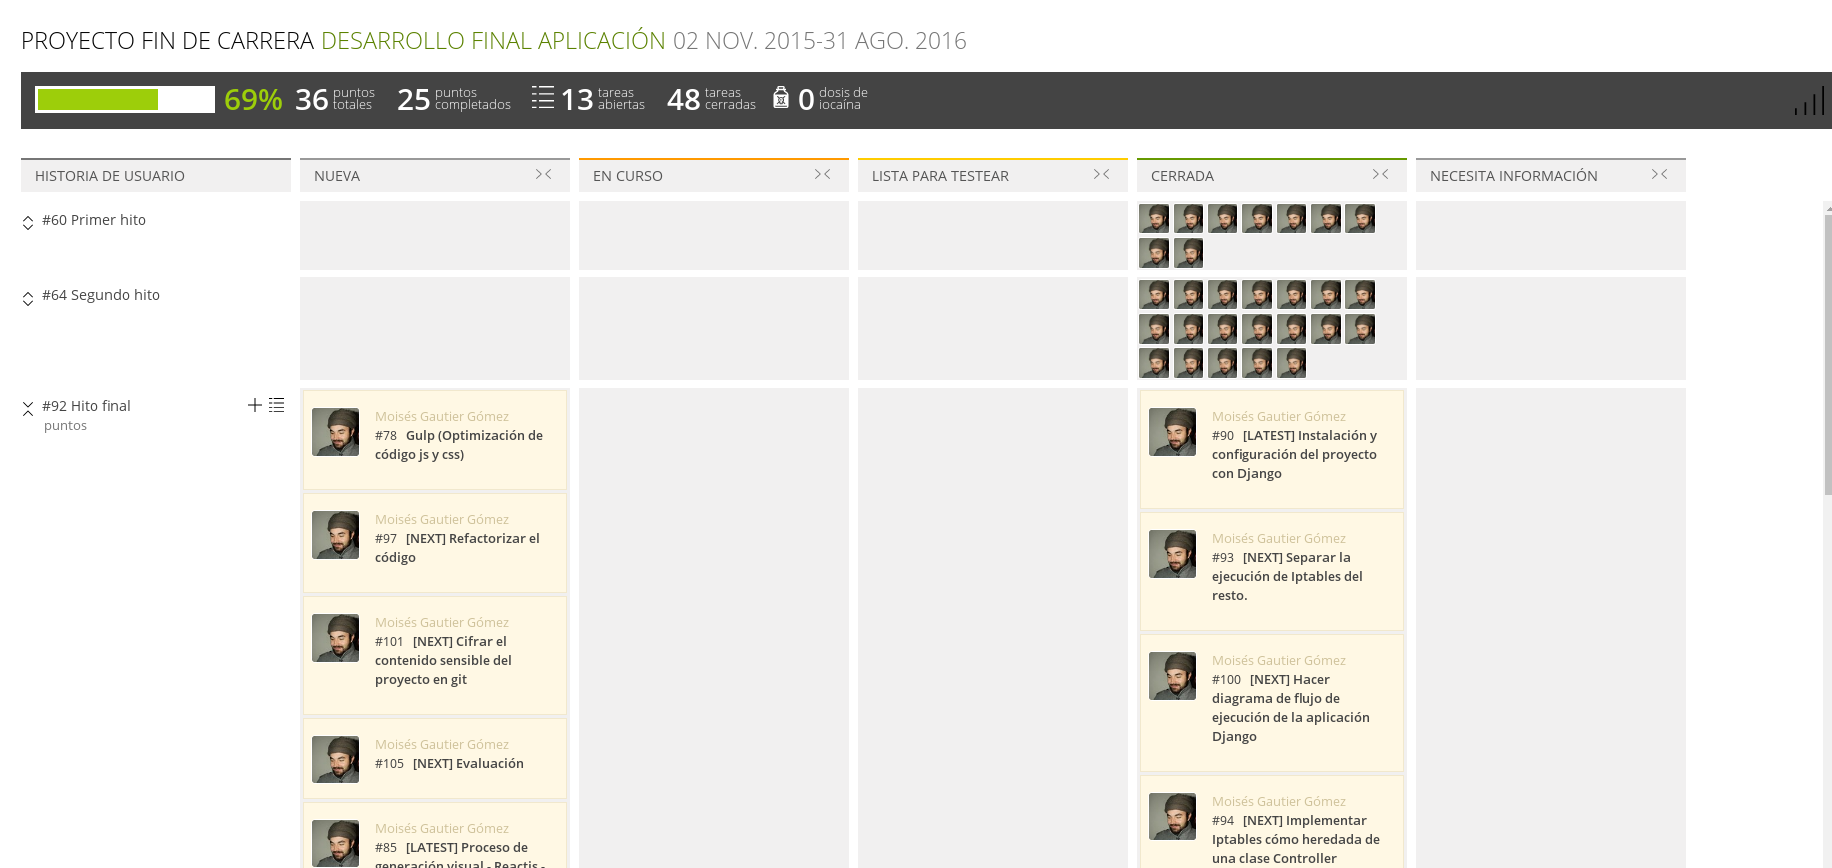
\includegraphics[scale=0.25]{diagramas/hito-taiga.png}}
\caption{Panel de actividades - Taiga}
\end{figure}

Los puntos más importantes del proyecto se han dividido en hitos, así como entregas que se definieron en cada reunión que se realizaba con el director del proyecto. También se ha definido una planificación temporal del desarrollo del proyecto mediante un diagrama de gantt con la duración de las tareas definidas en el panel de actividades de Taiga.\\
\section[Planificación temporal de tareas]{Planificación temporal de tareas}
\sectionmark{Tareas}


\newpage
\begin{figure}[H]
  \vspace*{-.2in}{
\hspace*{-.1in}{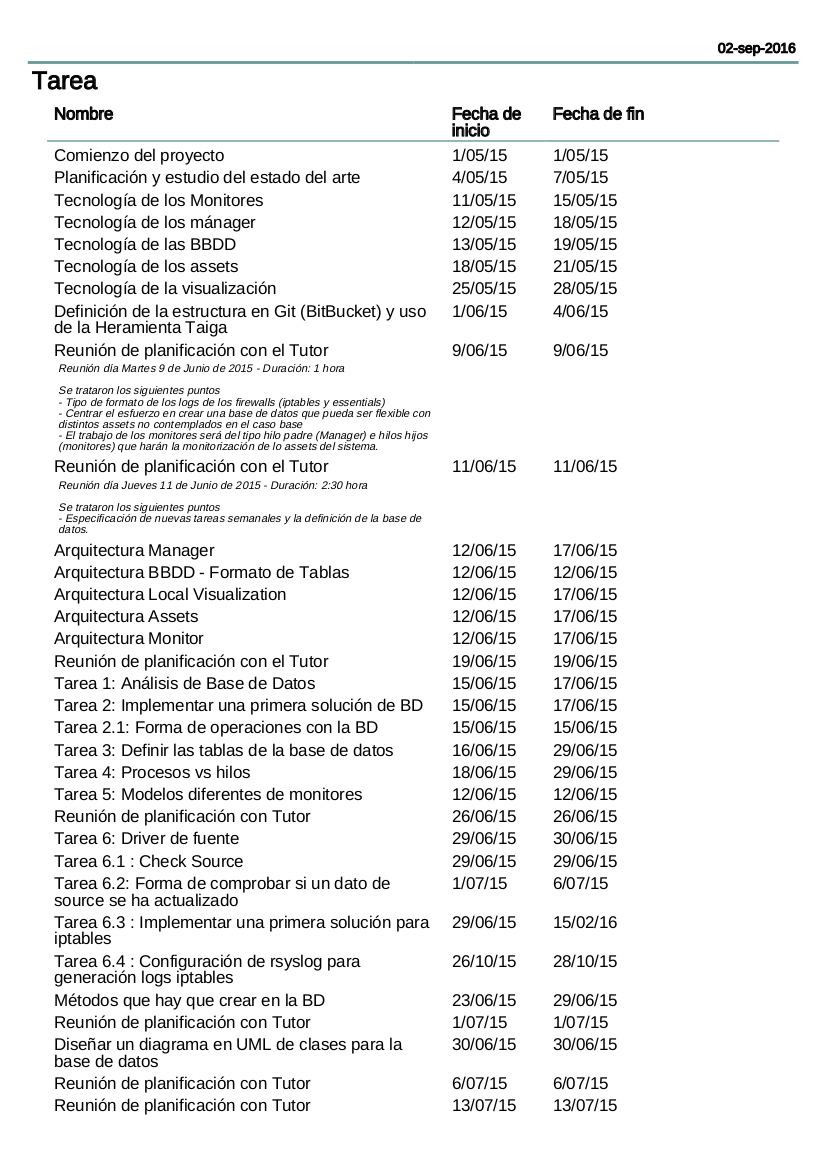
\includegraphics[scale=0.8]{diagramas/tareas-1.jpeg}}}
\caption{Primera tanda de tareas: 01-05-2015 a 13-07-2015}
\end{figure}
\newpage
\begin{figure}[H]
\hspace*{-.6in}{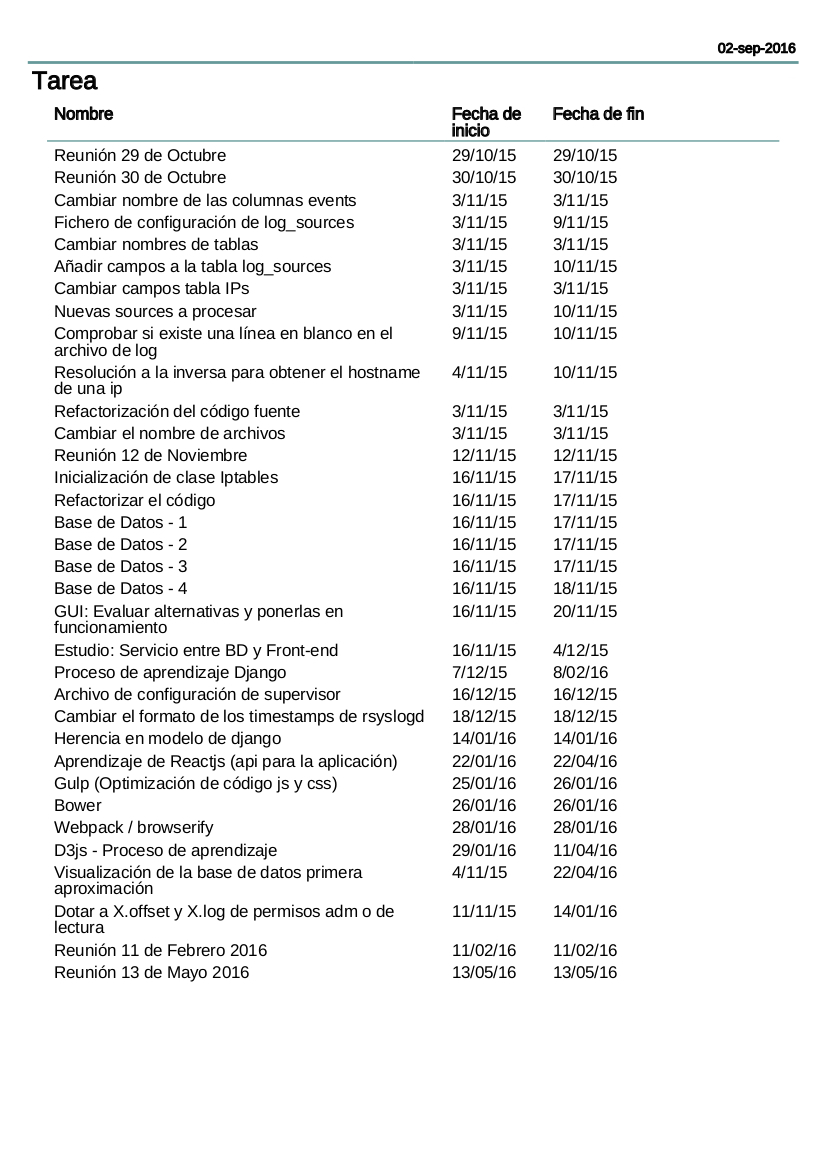
\includegraphics[scale=0.9]{diagramas/tareas-2.jpeg}}
\caption{Segunda tanda de tareas: 29-10-2015 a 25-04-2016}
\end{figure}
\newpage
\begin{figure}[H]
\hspace*{-.6in}{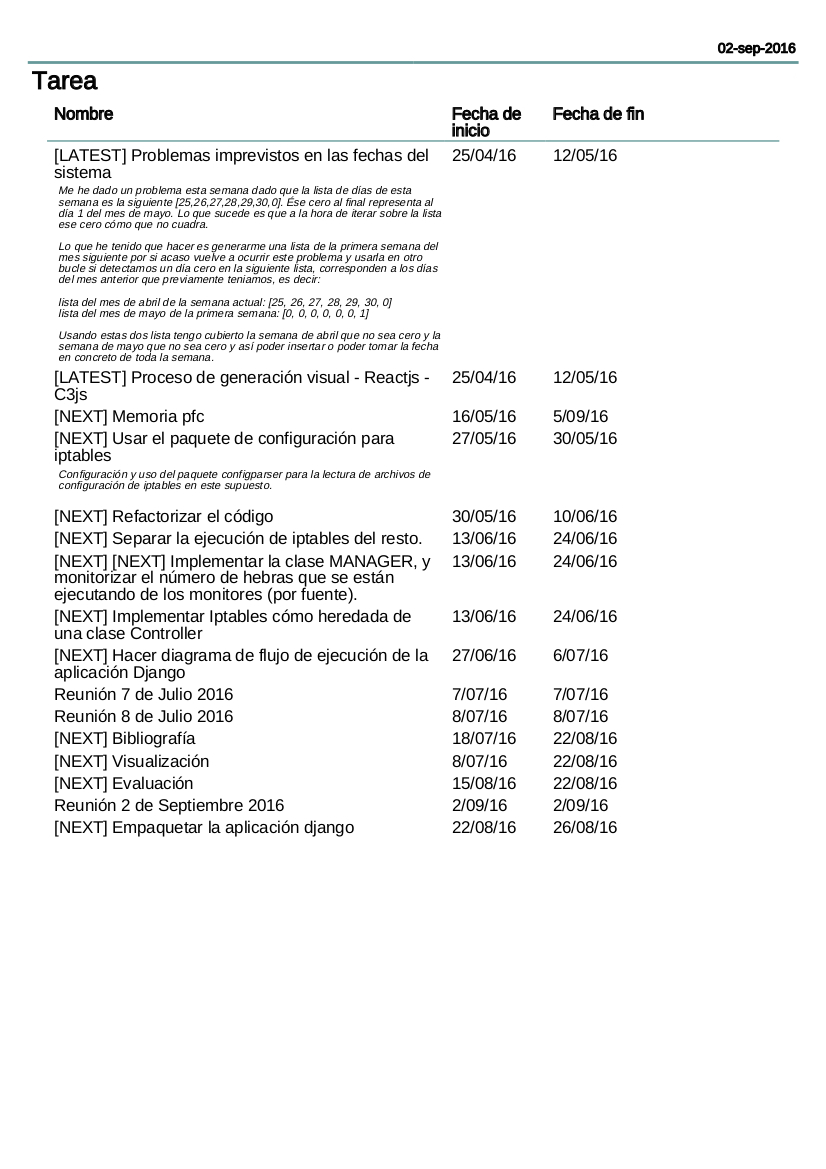
\includegraphics[scale=0.9]{diagramas/tareas-3.jpeg}}
\caption{Tercer tanda de tareas: 12-05-2016 a 06-09-2016}
\end{figure}
\newpage

\section{Diagrama de Gantt}
\begin{figure}[H]
\hspace*{1.5in}{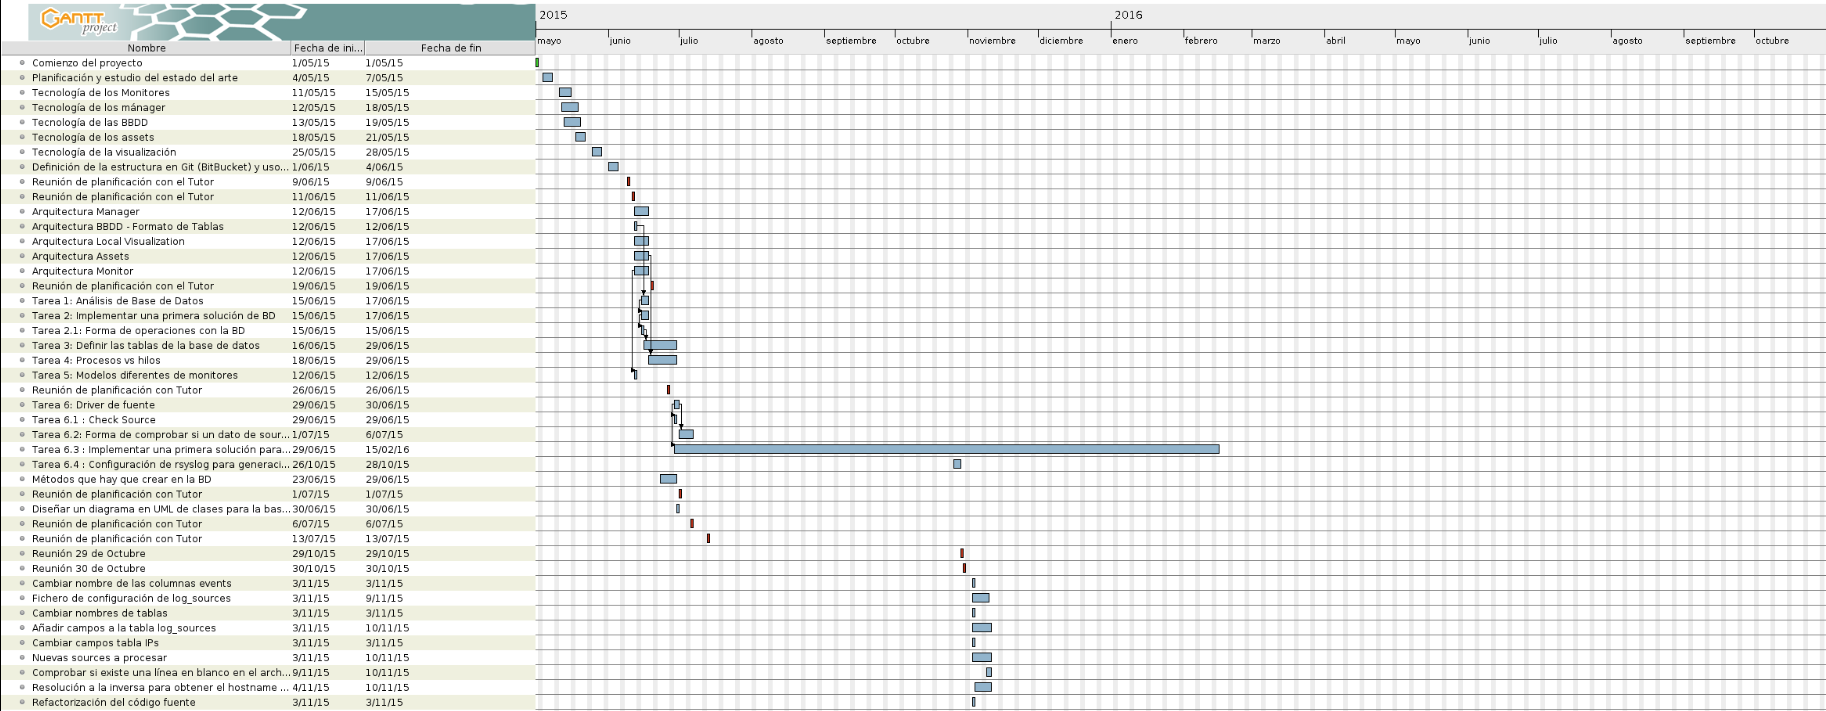
\includegraphics[scale=0.3,angle=270]{diagramas/gantt-1.png}}
\caption{Diagrama de Gantt 1-05-15 a 3-11-15}
\end{figure}
\newpage
\begin{figure}[H]
\hspace*{1.75in}{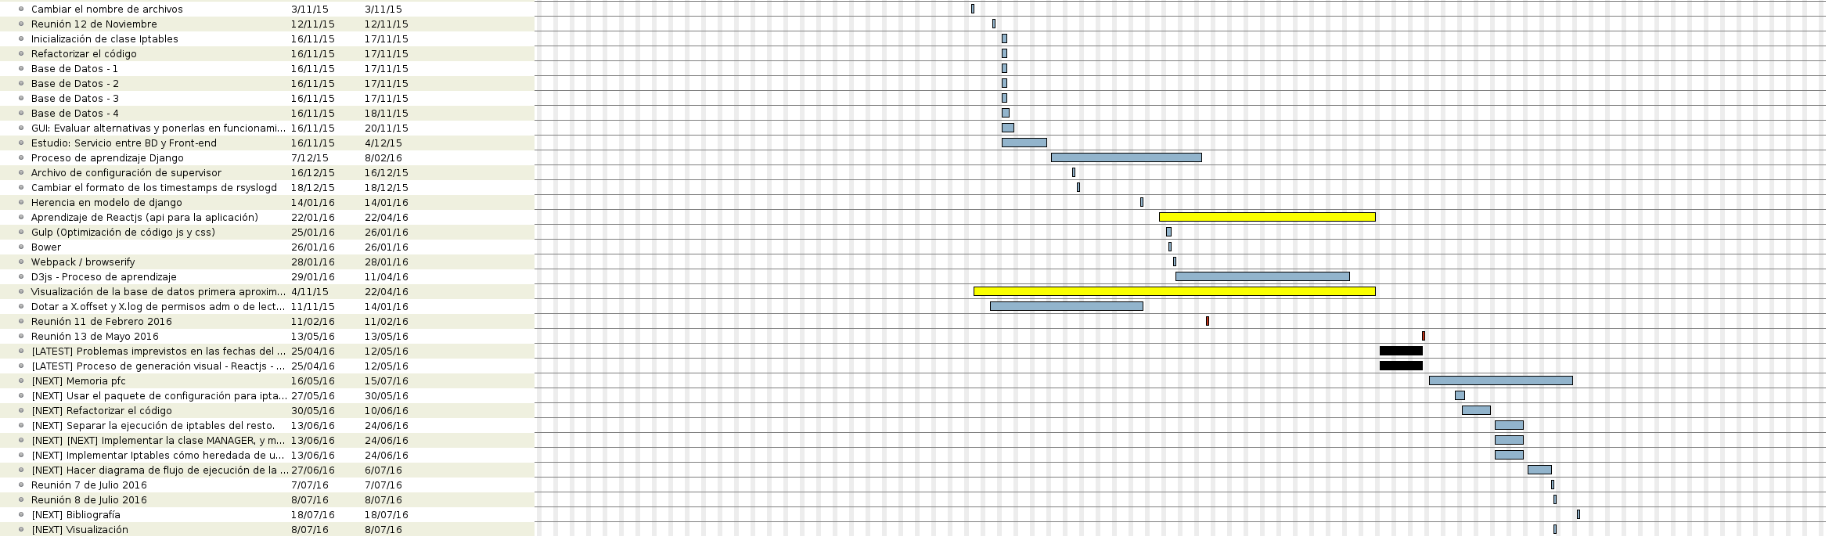
\includegraphics[scale=0.3,angle=270]{diagramas/gantt-2.png}}
\caption{Diagrama de Gantt 3-11-15 a 18-07-16}
\end{figure}
\newpage
